%%%%%%%%%%%%%%%%%%%%%%%%%%%%%%%%%%%%%%%%%%%%%%%%%%%%%%%%%%%%%%%%%%%%%%
% How to use writeLaTeX: 
%
% You edit the source code here on the left, and the preview on the
% right shows you the result withi.n a few seconds.
%
% Bookmark this page and share the URL with your co-authors. They can
% edit at the same time!
%
% You can upload figures, bibliographies, custom classes and
% styles using the files menu.
%
%%%%%%%%%%%%%%%%%%%%%%%%%%%%%%%%%%%%%%%%%%%%%%%%%%%%%%%%%%%%%%%%%%%%%%

\documentclass[12pt]{article}

\usepackage{sbc-template}

\usepackage{graphicx,url}
\usepackage{amsthm}

%\usepackage[brazil]{babel}   
\usepackage[utf8]{inputenc}  

     
\sloppy

\title{Prova da NP Completude de
\\The Legend of Zelda: A Link to the Past}

\author{Gustavo Kundlatsch e Gustavo Raimundo}


\address{Departamento de Informática e Estatística (INE)
\\Universidade Federal de Santa Catarina(UFSC)}

\begin{document} 

\maketitle

\begin{abstract}
  This paper has the objective to prove the NP completude of the game The Legend of Zelda: a Link to The Past,
  a classic game of the serie, released for the Super Nintendo Entertainment System (SNES).
  That is, if the game was played by an algorithm, the complexity to solve certain problems
  during it's run would be NP-Complete, so the game as a whole is NP-Complete. For this, we 
  will use a proof framework, used to make similar proofs to other games of the same company.
\end{abstract}
     
\begin{resumo} 
  Este artigo tem como objetivo provar a NP completude do jogo The Legend Of Zelda: a Link to The Past,
  um dos clássicos da franquia, lançado para o Super Nintendo Entertainment System (SNES). 
  Isto é, caso fosse jogado por um algoritmo, a complexidade
  para resolver certos problemas durante seu decorrer são NP-Completo, e assim,
  o jogo como um todo pode ser dito NP-Completo. Para isso, utilizaremos um framework
  que é utilizado para realizar provas semelhantes em diversos jogos da mesma empresa.
\end{resumo}

\section{Introdução}

Dentro da Inteligência Artificial (IA), agentes inteligentes são entidades capazes de raciocinar a respeito do ambiente em que estão inseridos e tomar decisões baseadas na situação em que se encontram \cite{russell2016artificial}. Dessa maneira, podemos descrever um agente pelo seus processos de percepção, raciocínio e atuação. O agente ocupa um ambiente, do qual recebe informações e no qual atua. O ambiente é o mundo em que o agente está inserido, podendo ser uma construção virtual como uma simulação ou uma parte do mundo real, no caso de um agente físico. Existem diversos tipos de ambientes que podem ser classificados de acordo com o seu fechamento (que determina se agentes de fora do ambiente podem afetar o sistema), dinamismo (a maneira como o ambiente evolui), determinismo (a consistência dos efeitos no ambiente) e cardinalidade (o número de objetos a serem afetados e percebidos) \cite{moya2007towards}.

Uma das maneiras de um agente atualizar seu conhecimento a respeito do ambiente é a percepção, o processo de utilizar sensores para detectar o ambiente e transformar os dados coletados em informações úteis \cite{weyns2004towards}.  O raciocínio, por sua vez, é o processamento das percepções baseado nos objetivos do agente, que resulta em um conjunto ações a serem tomadas através dos atuadores. O processo do raciocínio é comandado pela arquitetura cognitiva do agente, um modelo computacional inspirado na estrutura da mente humana \cite{DYACHENKO2018130}. As arquiteturas cognitivas podem ser divididas em três categorias: simbólicas, emergentes e híbridas \cite{yeCognitivearchitectures}. Arquiteturas simbólicas descrevem o ambiente através de símbolos armazenados em memória em uma base de conhecimentos, e utilizam lógica simbólica para realizar o ciclo de percepção, raciocínio e ação. Arquiteturas emergentes se baseiam na estrutura biológica do cérebro e normalmente utilizam redes neurais em uma estrutura hierárquica para lidar com situações de incerteza. Por fim, arquiteturas híbridas combinam o comportamento emergente e o processamento simbólico para resolver problemas de diversos domínios. 

Todavia, sensores podem apresentar problemas para o processo de percepção por razões como campo de visão, distância do objeto observado, resolução dos sensores e leituras não confiáveis \cite{chrisman1991intelligent}. Tratar deste problema normalmente é responsabilidade da arquitetura cognitiva do agente, pois a arquitetura precisa ser capaz de fazer a ponte entre o ambiente e o conhecimento do agente \cite{langley2009cognitive}.

O objetivo deste trabalho é apresentar um modelo genérico (independente da arquitetura do agente) que pode ser acoplado entre o processo de percepção e raciocínio, capaz de detectar e tratar percepções inválidas para transformá-las em informações úteis através de um processo de criação de novos planos. Esse modelo pressupõe um ambiente aberto (onde agentes externos podem influenciar o ambiente), dinâmico (mudanças no ambiente são causadas por eventos aleatórios) e não determinístico (ações do agente causam resultados diferentes no ambiente, mesmo em situações aparentemente idênticas, pois os resultados variam dependendo da percepção do agente daquele evento).  

\section{Apresentação dos Problemas}

Como a prova apresentada nesse artigo utiliza um framework, ela pode se
tornar um pouco abstrata demais. Nessa sessão apresentamos os problemas envolvidos e exemplos de cada um.

\subsection{The Legend of Zelda: a Link to The Past}

The Legend of Zelda: a Link to The Past é um jogo desenvolvido para Super Nintendo 
(que a partir desse momento será chamado apenas de Zelda, para facilitar a leitura), publicado pela
primeira vez em 1991, no Japão. Nele, controlamos o protagonista Link, um garoto que tem como objetivo
salvar a terra de Hyrule, impedir que o mago Ganon se torne o novo governante e salvar a princesa Zelda.
Para isso, Link deve obter a Triforce, uma relíquia sagrada espalhada pelo mapa, que é composta por 
três triângulos equiláteros, que trazem ao portador sabedoria, coragem e poder.

Em termos de design, o jogo é um mapa aberto, em que o jogador pode andar livremente. A câmera é posicionada acima
do plano, dando visão de uma parte do mapa total, sendo que quando o jogador se desloca para fora desse enquadramento
a câmera se desloca para exibir uma nova parte do mapa. O jogo é uma mistura de combates e puzzles. Para avançar
no jogo, é preciso explorar cavernas e construções, conversar com personagens e derrotar inimigos, assim obtendo
novos itens e habilidades. Os itens podem ser achados dentro de baús, sendo que existem itens especiais que quando são
encontrados seus baús permanecem abertos. Itens comuns podem voltam a ter seus baús fechados quando o jogador se move para
outro pedaço do mapa e retorna ao pedaço original (inimigos têm o mesmo comportamento, ou seja, a não ser que sejam chefes
especiais, os inimigos retornam ao mapa após morrerem caso haja essa troca de tela. Chefes especiais também liberam itens especiais).
Como Zelda é um jogo de mapa aberto, qualquer inimigo pode ser enfrentado a qualquer momento, desde que seja possível chegar até ele, dando grande liberdade ao jogador.

Tais itens e habilidades não são em si importantes para a prova que iremos realizar,
mas certamente poderiam ser utilizados para provar a NP-Completude por outros caminhos, como por exemplo realizando
uma redução ao problema 1-Push 2D \cite{demaine2000pushpush}.

\begin{figure}[!htb]
     \centering
     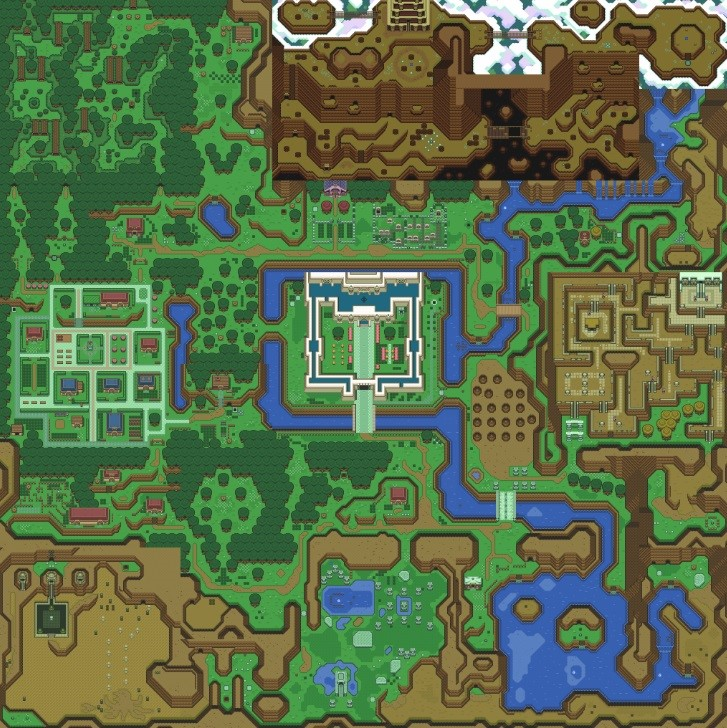
\includegraphics[scale=0.3]{zelda.jpg}
     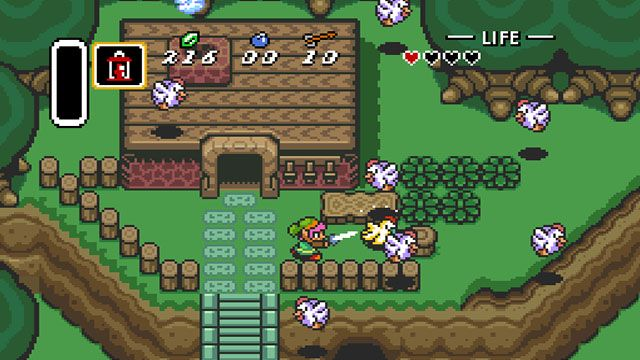
\includegraphics[scale=0.3]{link.jpg}
     \caption{Imagens do jogo}
\end{figure}

Diversos elementos do jogo podem ser utilizados para provar sua NP-Completude. Nesse jogo específico da franquia existe
um elemento bastante importante para esta prova, que o diferencia de seus anteriores: um gancho que Link pode utilizar
para se mover em direção a qualquer bloco do cenário.

\begin{figure}[!htb]
     \centering
     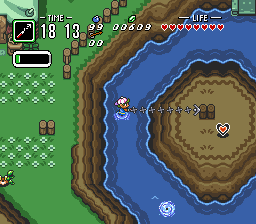
\includegraphics[scale=0.8]{hookshot.png}
     \caption{Exemplo de uso do gancho}
\end{figure}

\subsection{3-SAT}

O problema de satisfazibilidade booleana (SAT) é um problema de decisão, cuja instancia é uma escrita com operadores lógicos AND, OR, NOT, variáveis, e parênteses. A questão desse problema de decisão é: dada uma expressão, há alguma atribuição de valores verdadeiros e falsos para as variáveis que torne toda a expressão verdadeira? Uma fórmula da lógica proposicional é dita satisfazível se e somente se é possível atribuir valores lógicos a suas variáveis de tal maneira que eles tornem a fórmula verdadeira. A prova da NP Completude do problema SAT é dada pelo teorema de Cook-Levin \cite{cook1971complexity}.

O problema 3-SAT é um subconjunto do problema SAT, onde cada expressão lógica terá apenas três literais.

\begin{figure}[!htb]
     \centering
     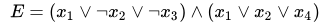
\includegraphics[scale=0.8]{cook.png}
     \caption{Exemplo do problema 3-SAT}
\end{figure}

\section{Framework}

O framework aqui apresentado foi originalmente proposto por \cite{aloupis2015classic}, e tem
como objetivo provar a NP-Hardness de jogos de plataforma. Para isso, ele implementa diversos dispositivos.
Apesar de The Legend of Zelda: a Link to The Past não ser um jogo de plataforma, mostraremos como ele se encaixa neste modelo.

\begin{figure}[!htb]
     \centering
     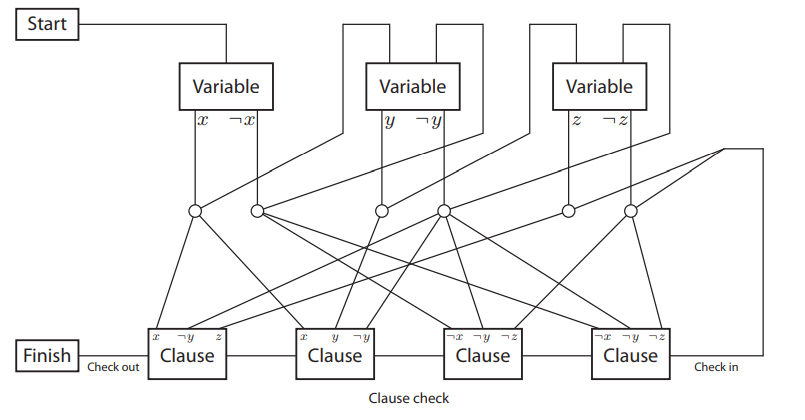
\includegraphics[scale=0.5]{framework.png}
     \caption{Framework geral para prova da NP Completude}
\end{figure}

Essa framework funciona da seguinte maneira: O jogador começa na posição Start. 
Cada dispositivo de variável obriga o jogador a fazer uma escolha
exclusiva de "verdadeiro" (\(x\)) ou "falso" (\(\lnot x\)) como valor para a variável para uma fórmula booleana. Ambas as escolhas
permitem ao jogador seguir caminhos que levam aos dispositivos de Cláusula, correspondentes as clausulas
que contém aquela literal (\(x\) ou \(\lnot x\)). Esses caminhos podem se cruzar, mas o dispositivo de Crossover
previne que o jogador troque entre caminhos cruzados. Ao visitar o dispositivo de cláusula, o jogador pode
desbloquear a cláusula (um estado permanente de mudança), mas não pode alcançar nenhum dos outros caminhos
conectados ao dispositivo de cláusula. Por fim, depois de atravessar através de todos os dispositivos de variáveis,
chegará a posição final. O jogador pode passear o caminho de checagem se e somente se cada cláusula for desbloqueada
por algum literal. Portanto, basta implementar os dispositivos citados para provar a NP-Hardness de qualquer jogo de plataforma.

Os dispositivos devem seguir as seguintes propriedades:

\textbf{Começo e Fim: } Os dispositivos de começo e fim contém o ponto inicial e o objetivo do personagem, respectivamente.

\textbf{Variável: }Cada dispositivo de variável precisa forçar o jogador a escolher um entre dois caminhos, correspondendo
a (\(xi\)) ou sua negação \(\lnot xi\) sendo escolhidos como o literal satisfeito, como por exemplo o caminho que foi escolhido ou o
caminho que não pode ser transposto. Cada dispositivo de variável deve ser acessível por apenas e tão somente o dispositivo de 
variável anterior, independentemente da escolha feita no dispositivo anterior, no qual o caminho a entrada de um literal não
permita a travessia de volta para a negação do literal.

\textbf{Cláusula e Checagem: }Cada dispositivo de cláusula deve ser acessível do (e inicialmente, apenas do) caminho vindo do
literal correspondente aos literais que aparecem na cláusula da fórmula Booleana. Além disso, quando um jogador
visita o dispositivo de cláusula dessa maneira, ele deve realizar alguma ação que "destrave" o dispositivo. O caminho de checagem
atravessa todo dispositivo de cláusula em sequência, e o jogador pode passar em todos os dispositivos de cláusula através do 
caminho de checagem se e apenas se o dispositivo de cláusula estiver desbloqueado. Assim o caminho de verificação pode ser
totalmente atravessado apenas se todos os dispositivos de variável tiverem sido visitadas dos caminhos de literais. Se o jogador
atravessar todo o caminho de verificação, ele pode acessar o dispositivo de fim.

\textbf{Crossover: }O dispositivo Crossover deve permitir a travessia através de duas passagens que se cruzam,
de tal forma que não há vazamento entre elas.


\section{Prova da NP-Completude}

Para realizar a prova da NP-Completude de Zelda, vamos primeiro demonstrar que tal problema é
NP-Hard, reduzindo-o para o problema 3SAT. Depois, mostraremos que é NP. Como por definição o conjunto
de problemas NP-Completo é a intersecção dos conjuntos de problemas NP com o conjunto de problemas NP-Hard,
teremos provado que Zelda é NP-Completo.

\subsection{NP-Hard}

\newtheorem*{theorem}{Teorema 1}

\begin{theorem}
    É NP-Hard decidir quando uma posição final é alcançável a partir de uma dada posição
    inicial em uma versão generalizada de The Legend Of Zelda: A Link to the Past.
\end{theorem}


\begin{proof}
    Existem várias maneiras de demonstrar esse teorema, uma vez que se uma parte do jogo
    for NP-Completa, todo o jogo também será. Para isso, utilizaremos apenas baús de tesouro
    e blocos, que servirão como alvo do gancho (vamos assumir que Link começa com esse item).
    Para realizar a prova, basta descrevermos o ambiente do jogo de acordo com os dispositivos
    do framework apresentado. Como esse não é um jogo de plataforma, não precisamos de um dispositivo
    específico de começo e fim, podendo o começo ser uma posição arbitrária dentro de uma caverna
    (onde normalmente ficam os puzzles que precisam do gancho) e uma posição arbitrária do mapa aberto,
    respectivamente.
    
    O dispositivo de variável, mostrado na figura 4, funciona da seguinte maneira: Link se aproxima ou
    do canto superior esquerdo ou do canto superior direito, dependendo de qual valor foi escolhido na
    variável anterior. Então Link usa o gancho para ir até um baú no centro superior, e por fim utiliza o
    gancho em um dos dois baús de baixo. Uma vez que Link alcançou um dos baús de baixo, o outro se torna
    inalcançável. Observe como diversas barreiras ao redor dos corredores impedem link de usar o gancho em outros
    baús de direções indesejáveis.
    
    \begin{figure}[!htb]
        \centering
        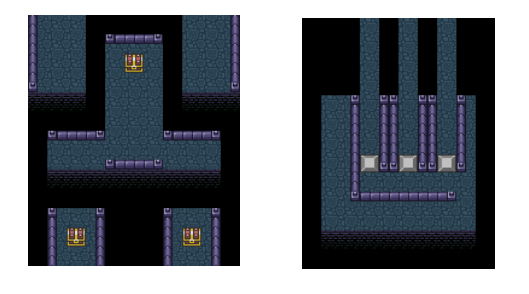
\includegraphics[scale=0.8]{proof1.png}
        \caption{Dispositivos de variável e cláusula, respectivamente}
    \end{figure}
    
    O dispositivo de cláusula é ilustrado também na figura 4. Os três corredores de cima correspondem aos literais que aparecem
    na cláusula. Quando link visita um desses corredores, ele deve empurrar o bloco para frente, o que permite a ele 
    utilizar o gancho em um dos blocos da direita depois, quando estiver atravessando o caminho de checagem (figura 5).
    Note que a barreira mais a esquerda do dispositivo de cláusula previne Link de "pular" clausulas não satisfeitas, mesmo
    se ele puder usar o gancho arbitrariamente a longas distâncias.
    
    \begin{figure}[!htb]
        \centering
        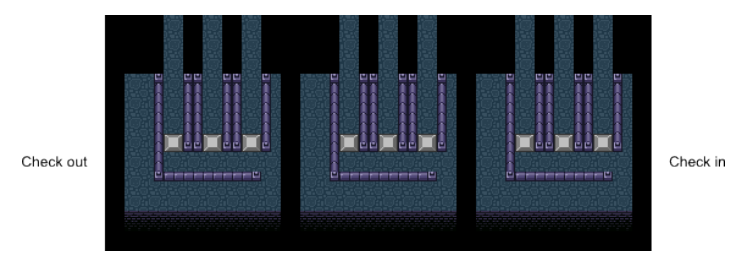
\includegraphics[scale=0.7]{proof2.png}
        \caption{Caminho de checagem}
    \end{figure}
    
    Por fim, o dispositimo de crossover já é nativamente implementado no jogo, como mostra a figura 6.
    
    \begin{figure}[!htb]
         \centering
         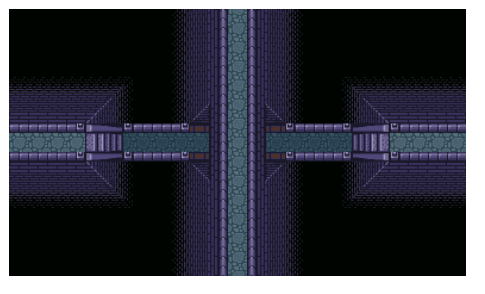
\includegraphics[scale=0.7]{proof3.png}
         \caption{Dispositivo de Crossover}
    \end{figure}
    
\end{proof}

\subsection{NP}

\newtheorem*{theorem2}{Teorema 2}

\begin{theorem2}
    Decidir quando uma posição final é alcançável a partir de uma dada posição
    inicial em uma versão generalizada de The Legend Of Zelda: A Link to the Past é NP.
\end{theorem2}

\begin{proof}
    Para concluir a prova da NP-Completude de Zelda, basta provarmos que finalizar o jogo é um problema NP.
    Se mostrarmos um caminho que é sempre possível,
    então há um algoritmo de solução de localização de caminho com um tempo de execução que é
    no máximo polinomial no tamanho da entrada, ou seja,
    podemos mostrar por certificados que o problema é verificável em tempo polinomial, o que por definição o torna um problema NP.
    
    Então, suponde que existe tal solução, vamos considerar qualquer caminho que Link pode fazer no mapa.
    Uma vez que só é possível abrir os baús que contém itens únicos do jogo uma vez, e que se matarmos
    todos os inimigos pelo menos uma vez teremos matado todos os inimigos que soltam itens especiais e também o chefe final do jogo, podemos dizer que
    o caminho que passa por cada um dos baús atualmente alcançáveis, e elimina cada um dos inimigos alcançáveis
    uma vez (lembrando que todos os inimigos podem ser derrotados desde o primeiro momento do jogo), então
    existe uma solução polinomial ao tamanho da entrada.
    
    Tal demonstração é similar as feitas por \cite{gabrielsen2012video} para outros jogos da Nintendo
    (Super Mario Bros., Donkey Kong Country e Metroid).

\end{proof}    



\section{Conclusões e Trabalhos Futuros}

A ideia desse trabalho foi fazer uma revisão sistemática da literatura até então existente, apresentação de um modelo genérico para implementar a solução proposta e ter uma discussão dos benefícios, desafios e do futuro de segurança em internet das coisas, em específico do uso de técnicas da blockchain para tratar desses problemas. 

O modelo apresentado, que descreve os sistemas apresentados na revisão sistemática, pode servir como base para diversas implementações de sistemas de segurança para redes de internet das coisas utilizando blockchain. Apesar de servir muito bem, e já ter sido provado eficiente através de implementações iniciais, ainda existem problemas a serem resolvidos na área como um todo. A maior dificuldade, sem dúvida, é o alto consumo energético, derivado do requisito computacional que os algoritmos de segurança blockchain requerem, além da memória utilizada. Apesar do resultado da implementação específica ter sido muito satisfatório tanto em custo computacional quanto em custo energético, mais estudo na área é necessário para poder se chegar a conclusões concretas e que abranjam de maneira mais geral modelos segurança para redes do tipo. Como os sensores e microprocessadores utilizados pelas ``coisas'' nas redes de IoT serem muito simples, com baixo potencial computacional, baixa memória e necessidade de baixo consumo energético por questões térmicas, muito dos algoritmos de blockchain precisam ser revistos para que esse tipo de solução se torne simples de ser implantada e comum de ser vista nas redes domésticas, industriais e científicas.

O principal trabalho discutido em nossa revisão, e que foi utilizado como base para montarmos uma proposta concreta de solução genérica de segurança para internet das coisas utilizando blockchain \cite{dorri2017blockchain}, mostra como é possível fazer implementações do tipo, pois no trabalho realmente foi feita uma rede completa de internet das coisas para que os testes fossem realizados, tanto com blockchain quanto sem blockchain. Apesar do exemplo com blockchain ter apresentado resultados espetaculares com um custo de energia bem reduzido e tempo de resposta adicional quase desconsideráveis, mesmo que maior do que a implementação sem blockchain, que em questão de segurança era muito inferior devido a natureza simples das verficações de segurança e confiabilidade da rede, a replicação em larga escala do mesmo modelo ainda assim poderia trazer problemas por conta de um crescimento linear do custo. Mesmo assim, esse trabalho é pioneiro na área de otimização do tipo de solução apresentada, e tende a ser um tipo de trabalho a se repetir em novas esferas, com contextos diferentes e implementações ainda mais otimizadas que vão tornar possível a indústria aplicar esse tipo de solução a qualquer rede de coisas inteligentes a serem vendidas para o usuário final.

Em nosso trabalho apresentamos um modelo genérico, que possui certa validação mas que ainda pode ser aprimorado e testado arduamente para conseguir dados mais objetivos e relevantes para que a proposta como um todo se concretize como uma solução válida e implementável para redes de diversos tamanhos. Caso isso não aconteça, é certo que para determinados tipos e tamanhos de redes de internet das coisas o modelo funciona, então mesmo assim pode ser utilizado, apenas em empreitadas específicas e talvez reduzidas.

Portanto, os trabalhos futuros devem almejar não só a corretude da solução proposta, com modelos que já foram apresentados como funcionais por trabalhos anteriores, mas também focar na otimização das soluções para que tenham necessidade de menor custo computacional e consumo energético, para que em aplicações de larga escala a solução utilizando blockchain continue viável, mesmo com possivelmente milhões de coisas inteligentes interconectadas. Uma alternativa para essa solução é investir em soluções distribuídas, onde a computação pode ser distribuída de maneira eficiente através de algoritmos de distribuição de carga entre os diversos microprocessadores da rede IoT, extraindo o máximo potencial que essa tecnologia tem a oferecer com sua natureza de muitos dispositivos com pouco potencial de computação individual.

Além do avanço no trabalho atual como citado no parágrafo anterior, a arquitetura apresentada, bem como as contribuições que ela traz para a segurança em internet das coisas mesclando o crescente uso de controladores inteligentes com conceitos como blockchain, podem ser ainda mais mesclados com conceitos avançados de computação, IoT ou segurança. Um exemplo claro disso é a possibilidade de aplicar a técnica de Fog computing no modelo apresentado. Essa adição está fora do escopo do trabalho realizado, mas combina perfeitamente com a ideia de reduzir custo computacional de maneira geral na rede de internet das coisas e nesse caso específico para reduzir o custo computacional da implementação do Blockchain em um ambiente com diversos sensores transmitindo um grande volume de dados constantemente.

Por último, vale ressaltar a importância da transparência e da comunicação humana além das estratégias de segurança adotada. É crucial que o consumidor saiba que tipo de dados estão sendo coletados, e que tipo de sensores existem nos dispositivos inteligentes instalados em sua casa para que o relacionamento entre o consumidor e a rede utilizada seja saudável, despertando não só o interesse comercial com um aproveito unilateral por parte das empresas que provém esse tipo de serviço. Aviso da escolha, do mecanismo de acesso e da precisão da informação recolhida, políticas efetivas de minimização dos dados coletados e prestação de contas das medidas e falhas de segurança nos dispositivos são alguns fundamentos que tem se mostrado tendência por empresas que presam por um relacionamento saudável com o consumidor.


%\section*{Agradecimentos}

\bibliographystyle{sbc}
\bibliography{sbc-template}

\end{document}
